\documentclass[12pt]{article}
\usepackage{blindtext}
\usepackage{geometry}
\geometry{
	a4paper,
	left=40mm,
	right=15mm,
	top=30mm,
	bottom=35mm,
 }
\usepackage{setspace}
% Seznam balíků
\usepackage{comment}
\usepackage{lmodern}
\usepackage{cmap}
\usepackage[czech]{babel}
\usepackage[T1]{fontenc}
\usepackage[utf8]{inputenc}
\usepackage{graphicx}
\usepackage{epstopdf}
\usepackage{makeidx}
\usepackage{listings}
\usepackage[export]{adjustbox}
\usepackage[font=scriptsize,labelfont=bf]{caption}
\usepackage{booktabs}
\usepackage{subcaption}
\usepackage{array}
\usepackage{multirow}
\usepackage{enumitem}
\usepackage{tocbibind}
\usepackage{courier}
\usepackage{pdfpages}
\usepackage{hyperref}
\hypersetup{
	colorlinks,
	citecolor=black,
	filecolor=black,
	linkcolor=black,
	urlcolor=black
}

% Začátek dokumentu
\begin{document}
	% Titulní stránka
	\begin{titlepage}
		\centering
		\begin{tabular}{m{0.2\linewidth}m{0.8\linewidth}}
			
\includegraphics[width=\linewidth]{SPSE_logo.png}
			&\centering
			\textbf{Vyšší odborná škola}\par
			\textbf{a Střední průmyslová škola elektrotechnická}\par
			\textbf{Plzeň, Koterovská 85}
		\end{tabular}
		\centering
		\vfill
		{\Huge\scshape Ročníková práce\par}
		\raggedright
		\vspace{4cm}
		{\Large Téma: Programovatelné auto\par}
		\vfill
		
		% Spodní část titulní stránky
		\begin{tabular}{ll}
			Autor práce:		&	Jan Ocelík \\
			Obor studia:		&	78-42-M/01 Technické lyceum \\
			Třída:				&	3. L \\
			Předmět:			&	Kybernetika \\
			Zadávající učitel:	&	Jiří Švihla \\
			Dne:				&	28. 4. 2023 \\
								&	\\
			Hodnocení:			&	\\
		\end{tabular}
	\end{titlepage}

	% Zadání
	\thispagestyle{empty}
	\includepdfset{offset=15mm 0mm,noautoscale,pages={-},pagecommand={}}
	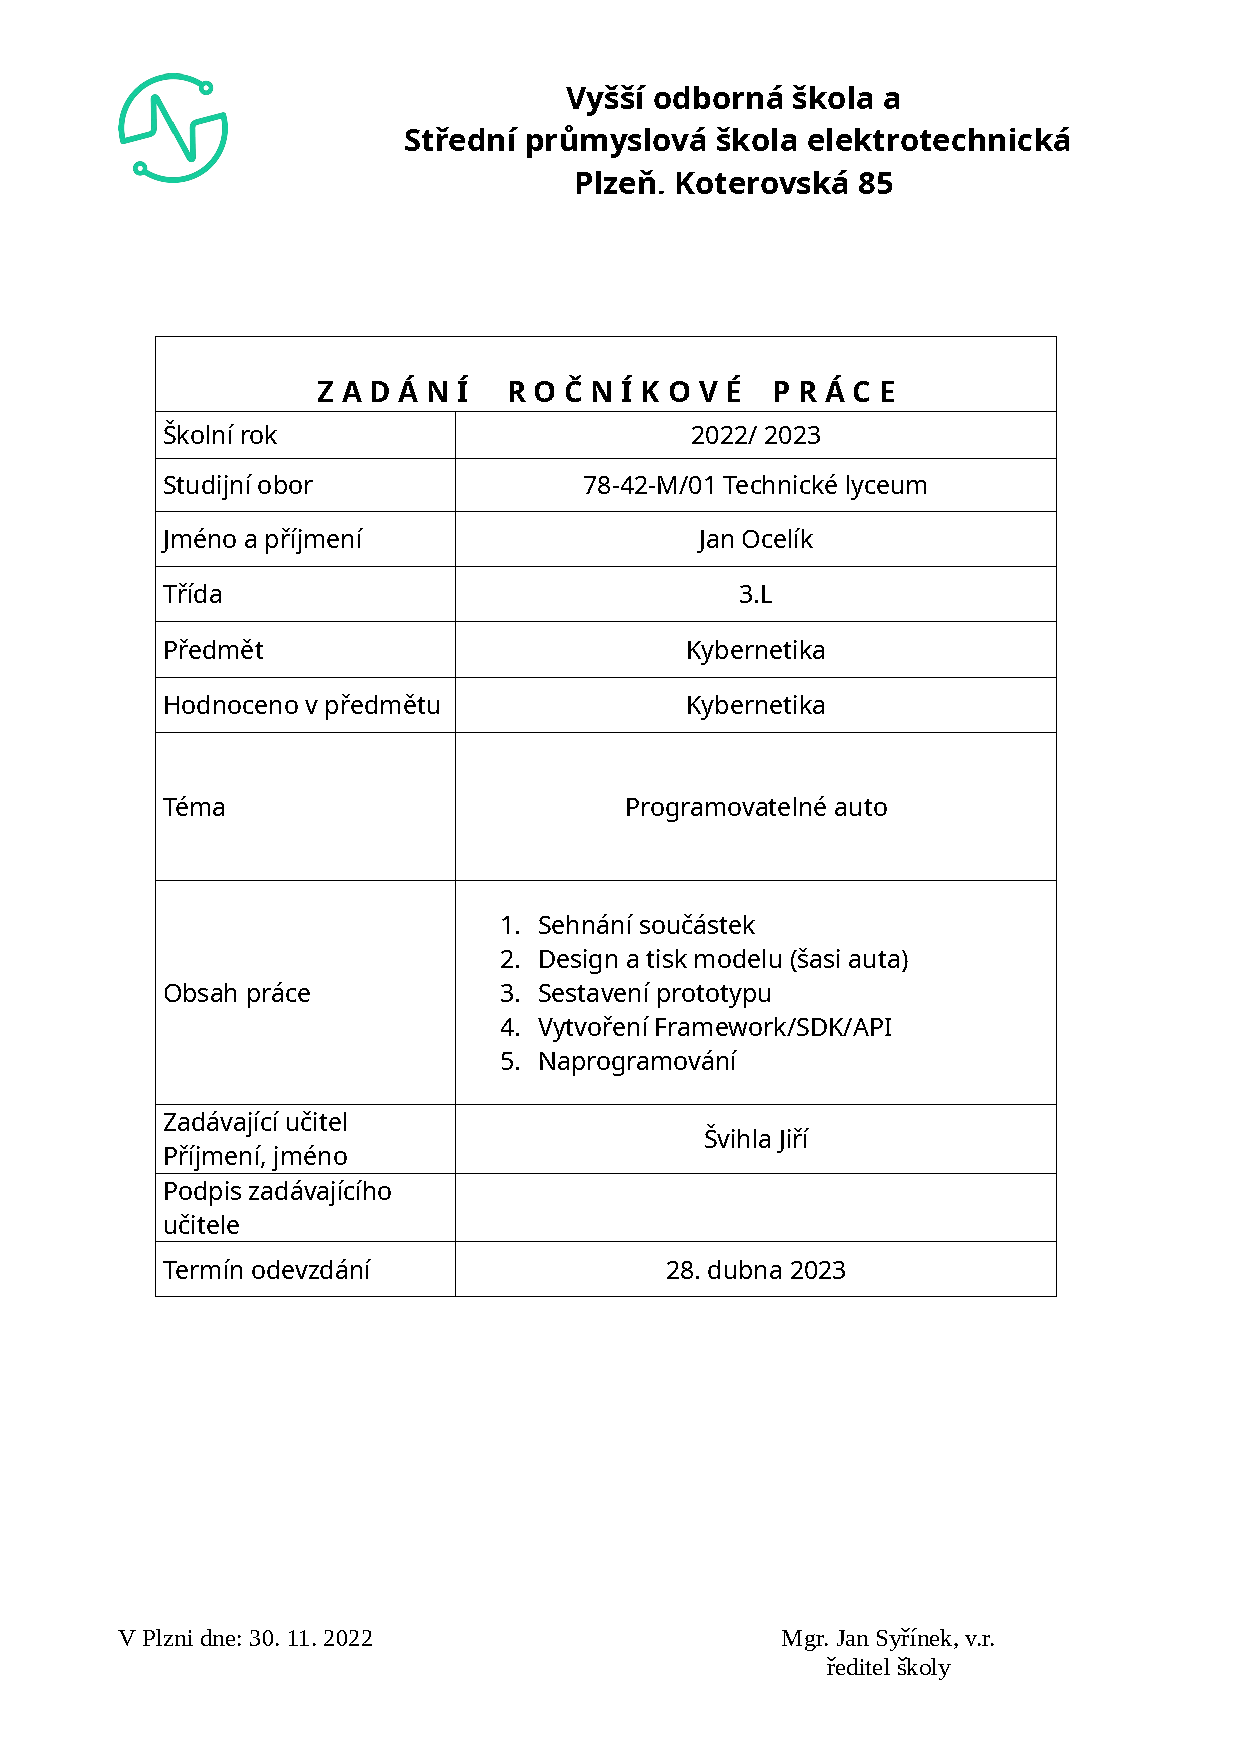
\includepdf[pages=1]{Zadani_RP_TL_22_23.pdf}
	
	\begin{spacing}{1.5}
	
	% Anotace
	\newpage
	\thispagestyle{empty}
	\section*{Anotace}
	\addcontentsline{toc}{section}{Anotace}
	\paragraph{} Cílem této ročníkové práce je za pomoci opensource programů navrhnout a z opensource komponent poskládat robotické autíčko pro začátečníky i pokročilé s možností jednoduchého sestavení. Dalším úkolem je vyvinout firmware a API pro jednoduché skriptové programovaní i komplexnější programování s využitím obrazového vstupu. Dalším úkolem je připravit ukázkové příklady kódu k předvedení jednotlivých funkcí robota. Posledním úkolem je zpříjemnit práci s robotem, zhodnotit přínosy a možnosti využití projektu ve vzdělávání a vypracovat potřebnou dokumentaci.
	\vfill
	\paragraph{} „Prohlašuji, že jsem tuto práci vypracoval samostatně a použil literárních pramenů a informací, které cituji a uvadím v seznamu použité literatury a zdrojů informací.“
	\paragraph{} „Souhlasím s využitím mé práce učteli VOŠ a SPŠE Plzeň k výuce.“
	\paragraph{} \hfill Plzni dne: .................... Podpis: ....................
	
	% Poděkování
	\newpage
	\thispagestyle{empty}
	\section*{Poděkování}
	\addcontentsline{toc}{section}{Poděkování}
	\paragraph{} Tímto bych chtěl poděkovat vedoucímu práce Jiřímu Švihlovi za pomoc s výběrem komponent a obsahem dokumentace a rodině a přátelům za psychickou podporu. Také děkuji všem dohromady za to, že mě k tomu včas dokopali.
	
	% Obsah
	\newpage
	\tableofcontents
	
	% Úvod
	\newpage
	\section*{Úvod}
	\addcontentsline{toc}{section}{Úvod}
	\paragraph{} V dnešní době se stále více hovoří o automatizaci a digitalizaci a tyto trendy mají velký vliv na společnost. Robotika a autonomní systémy jsou jednou z klíčových oblastí, které se rozvíjejí v rámci těchto trendů a mají potenciál změnit mnoho aspektů našeho života.
	\paragraph{} Vzdělávání a výuka v této oblasti se také stávají stále důležitějšími, protože mnoho pracovních pozic, které budou v budoucnosti vyžadovat znalosti robotiky a programování, ještě neexistuje. Výuka v této oblasti tak může být klíčová pro přípravu studentů na pracovní trh budoucnosti.
	\paragraph{} Proto jsem se rozhodl věnovat svou ročníkovou práci právě problematice robotiky a vytvořit autonomní auto, které bude sloužit jako výuková pomůcka. Můj záměr je ukázat, jak moderní technologie mohou být využity k tomu, aby byly studenti lépe připraveni na budoucí výzvy v oblasti robotiky a informatiky.
	\paragraph{} Při tvorbě prototypu se budu snažit využít nejnovější poznatky v oblasti robotiky a programování, a to jak z teoretického hlediska, tak z praktického testování. Cílem bude vytvořit zařízení, které bude snadno ovladatelné a srozumitelné pro studenty různých věkových kategorií, a zároveň bude dostatečně funkční a výkonné pro splnění zadaných úkolů.
	\paragraph{} Věřím, že tato ročníková práce přispěje k popularizaci robotiky a podpoří zájem studentů o tuto oblast. Tím může mít pozitivní vliv na jejich budoucí kariéru a na rozvoj robotiky v České republice.
	
	% Cíle a požadavky
	\newpage
	\section{Cíle a požadavky}
	
	\subsection{Komponenty (Moduly)}
	\paragraph{} Hlavním cílem této ročníkové práce je návrh a výroba robota ze všem dostupných materiálů, v tomto případě ze snadno sehnatelných modulů.
	\paragraph{} Moduly by měly být zároveň opensource, aby si software pro ně mohl programovat každý, který se k robotovi dostane, nebo si ho sám vyrobí.
	\paragraph{} Důležitý je také výběr napájení, v případě robotického auta tedy baterie, tak, aby udrželo robota v provozu po přiměřeně dlouhou dobu a aby zároveň dokázalo vykrýt proudové špičky.
	
	\subsection{Šasi (tělo)}
	\paragraph{} Tělo robota by mělo být vyrobeno tak, aby bylo plně uzavíratelné, tedy bezpečné pro jakýkoli přenos i při nešetrném zacházení, ale aby se dal robot také provozovat s plně přístupnými veškerými propojkami a bylo tedy snadné ladit jeho hardware za provozu.
	
	\subsection{API}
	\paragraph{} Jedním z dalších požadavků je co nejvíce zpříjemnit uživateli práci s robotickým autem, tedy vytvořit nějaké API nebo knihovnu.
	\paragraph{} Nedílnou součástí je také dokumentace k danému API/knihovně a to proto, aby si i nově příchozí uživatel zvládl bez jakékoli pomoci robota pomocí daného API/knihovny naprogramovat.
	
	% Návrhový software
	\newpage
	\section{Návrhový software}
	
	\subsection{Onshape}
	\paragraph{} Onshape je online software pro návrh 3D součástí. V programu se vytváří takzvaný dokument, ve kterém se nadále dají zakládat \uv{studia}. Onshape nabízí mnoho zajímavých možností, typického uživatele však zajímají tato tři hlavní studia - \textbf{Part Stuido}, \textbf{Assembly} a \textbf{Drawing}.
	\subsubsection*{Part Studio}
	\paragraph{} Part Studio slouží, jak už název napovídá, k vytváření jednotlivých dílů. Díly se vytvářejí a upravují pomocí příkazů, jako například \textbf{Sketch}, sloužící k sestrojení 2D náčrtu, \textbf{Extrude}, k \uv{vytáhnutí} náčrtu do třetího rozměru, nebo \textbf{Fillet}, k zaoblení hran. Tyto příkazy lze vyvolat kliknutím na jejich ikonu v horní liště programu, přepsáním jejich názvu do \textbf{Search tools}, nebo, u některých více používaných, klávesovými zkratkami.
	
	\begin{figure}[h]
		\centering
		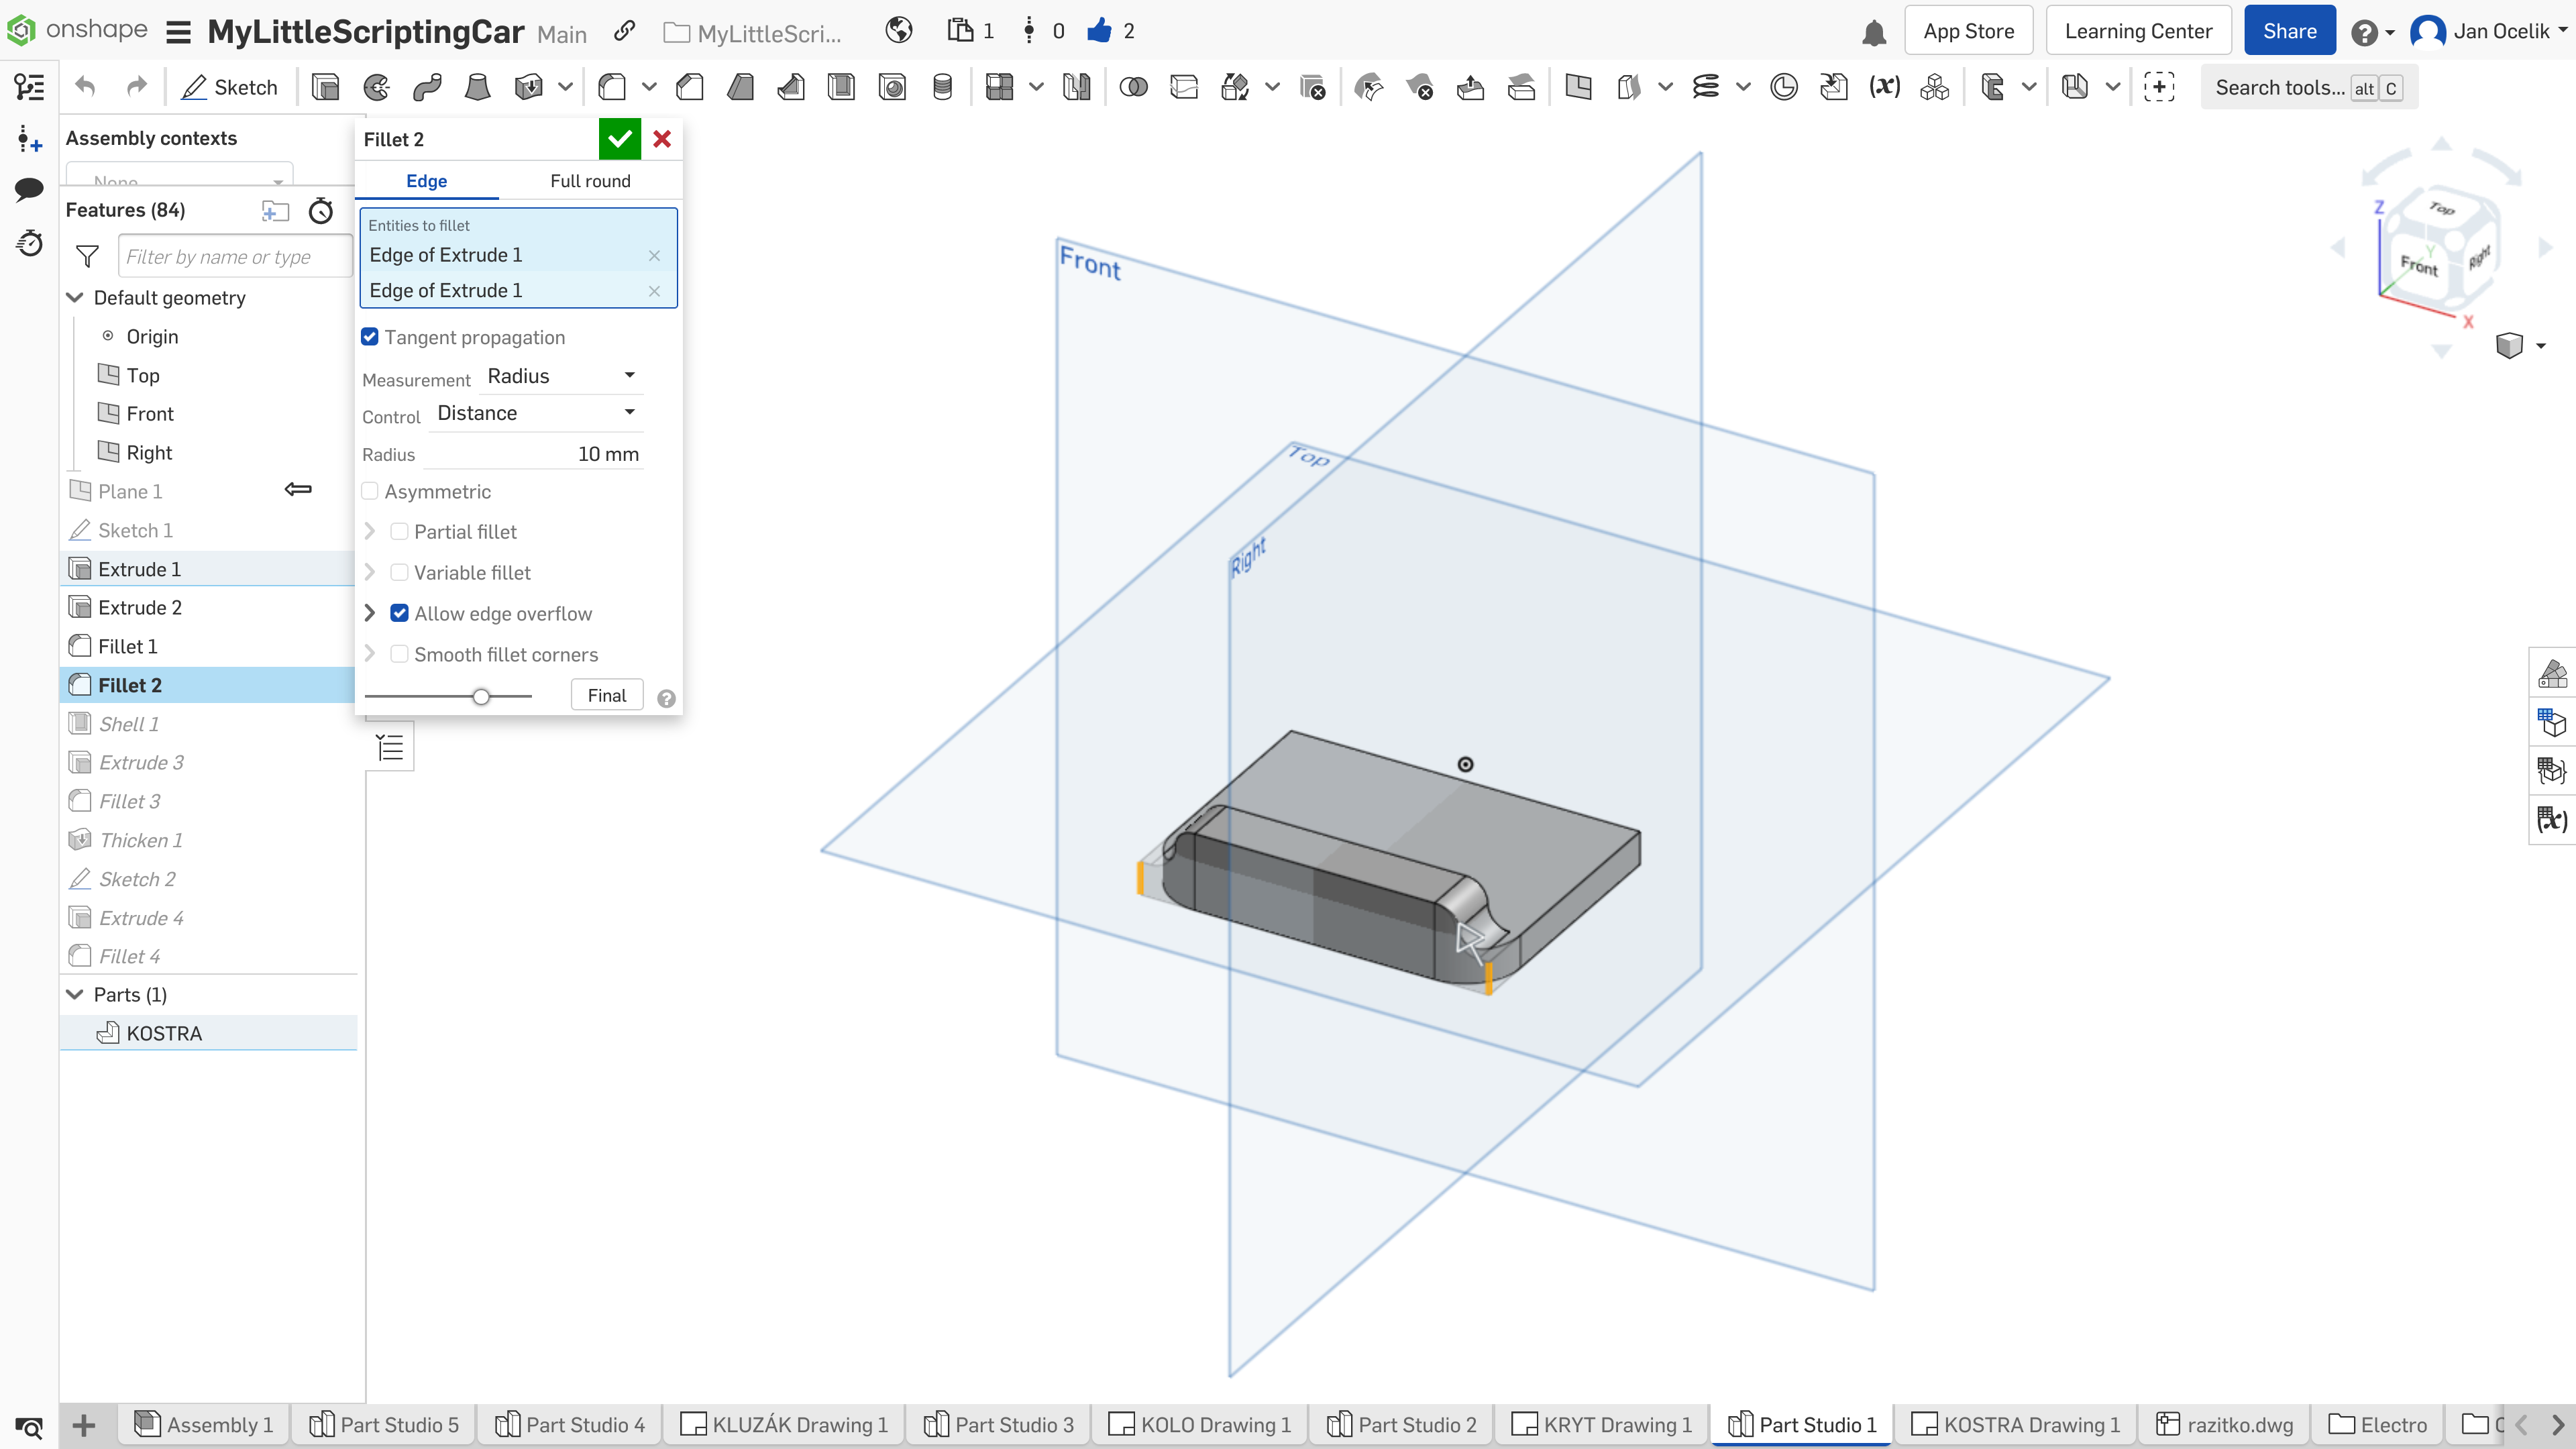
\includegraphics[width=\linewidth]{images/part_studio.png}
		\caption{Part Studio}
		\label{fig:part_studio}
	\end{figure}
	
	\subsubsection*{Assembly}
	\paragraph{} Další studio v programu Onshape, Assmebly, slouží ke spojování (nebo alespoň aranžování) jednotlivých dílů. K tomuto účelu slouží příkazy, které se, opět, nechají vyvolat několika způsoby, včetně klepnutím na ikonu v horní liště studia. Další výhodnou funkcí tohoto studia je \textbf{Create Part Studio in context}, což dělá přesně to, co se v názvu píše; vytvoří studio dílu v kontextu se sestavou. Tato funkce může hodně usnadnit vytváření některých dílů.
	
	\begin{figure}[h]
		\centering
		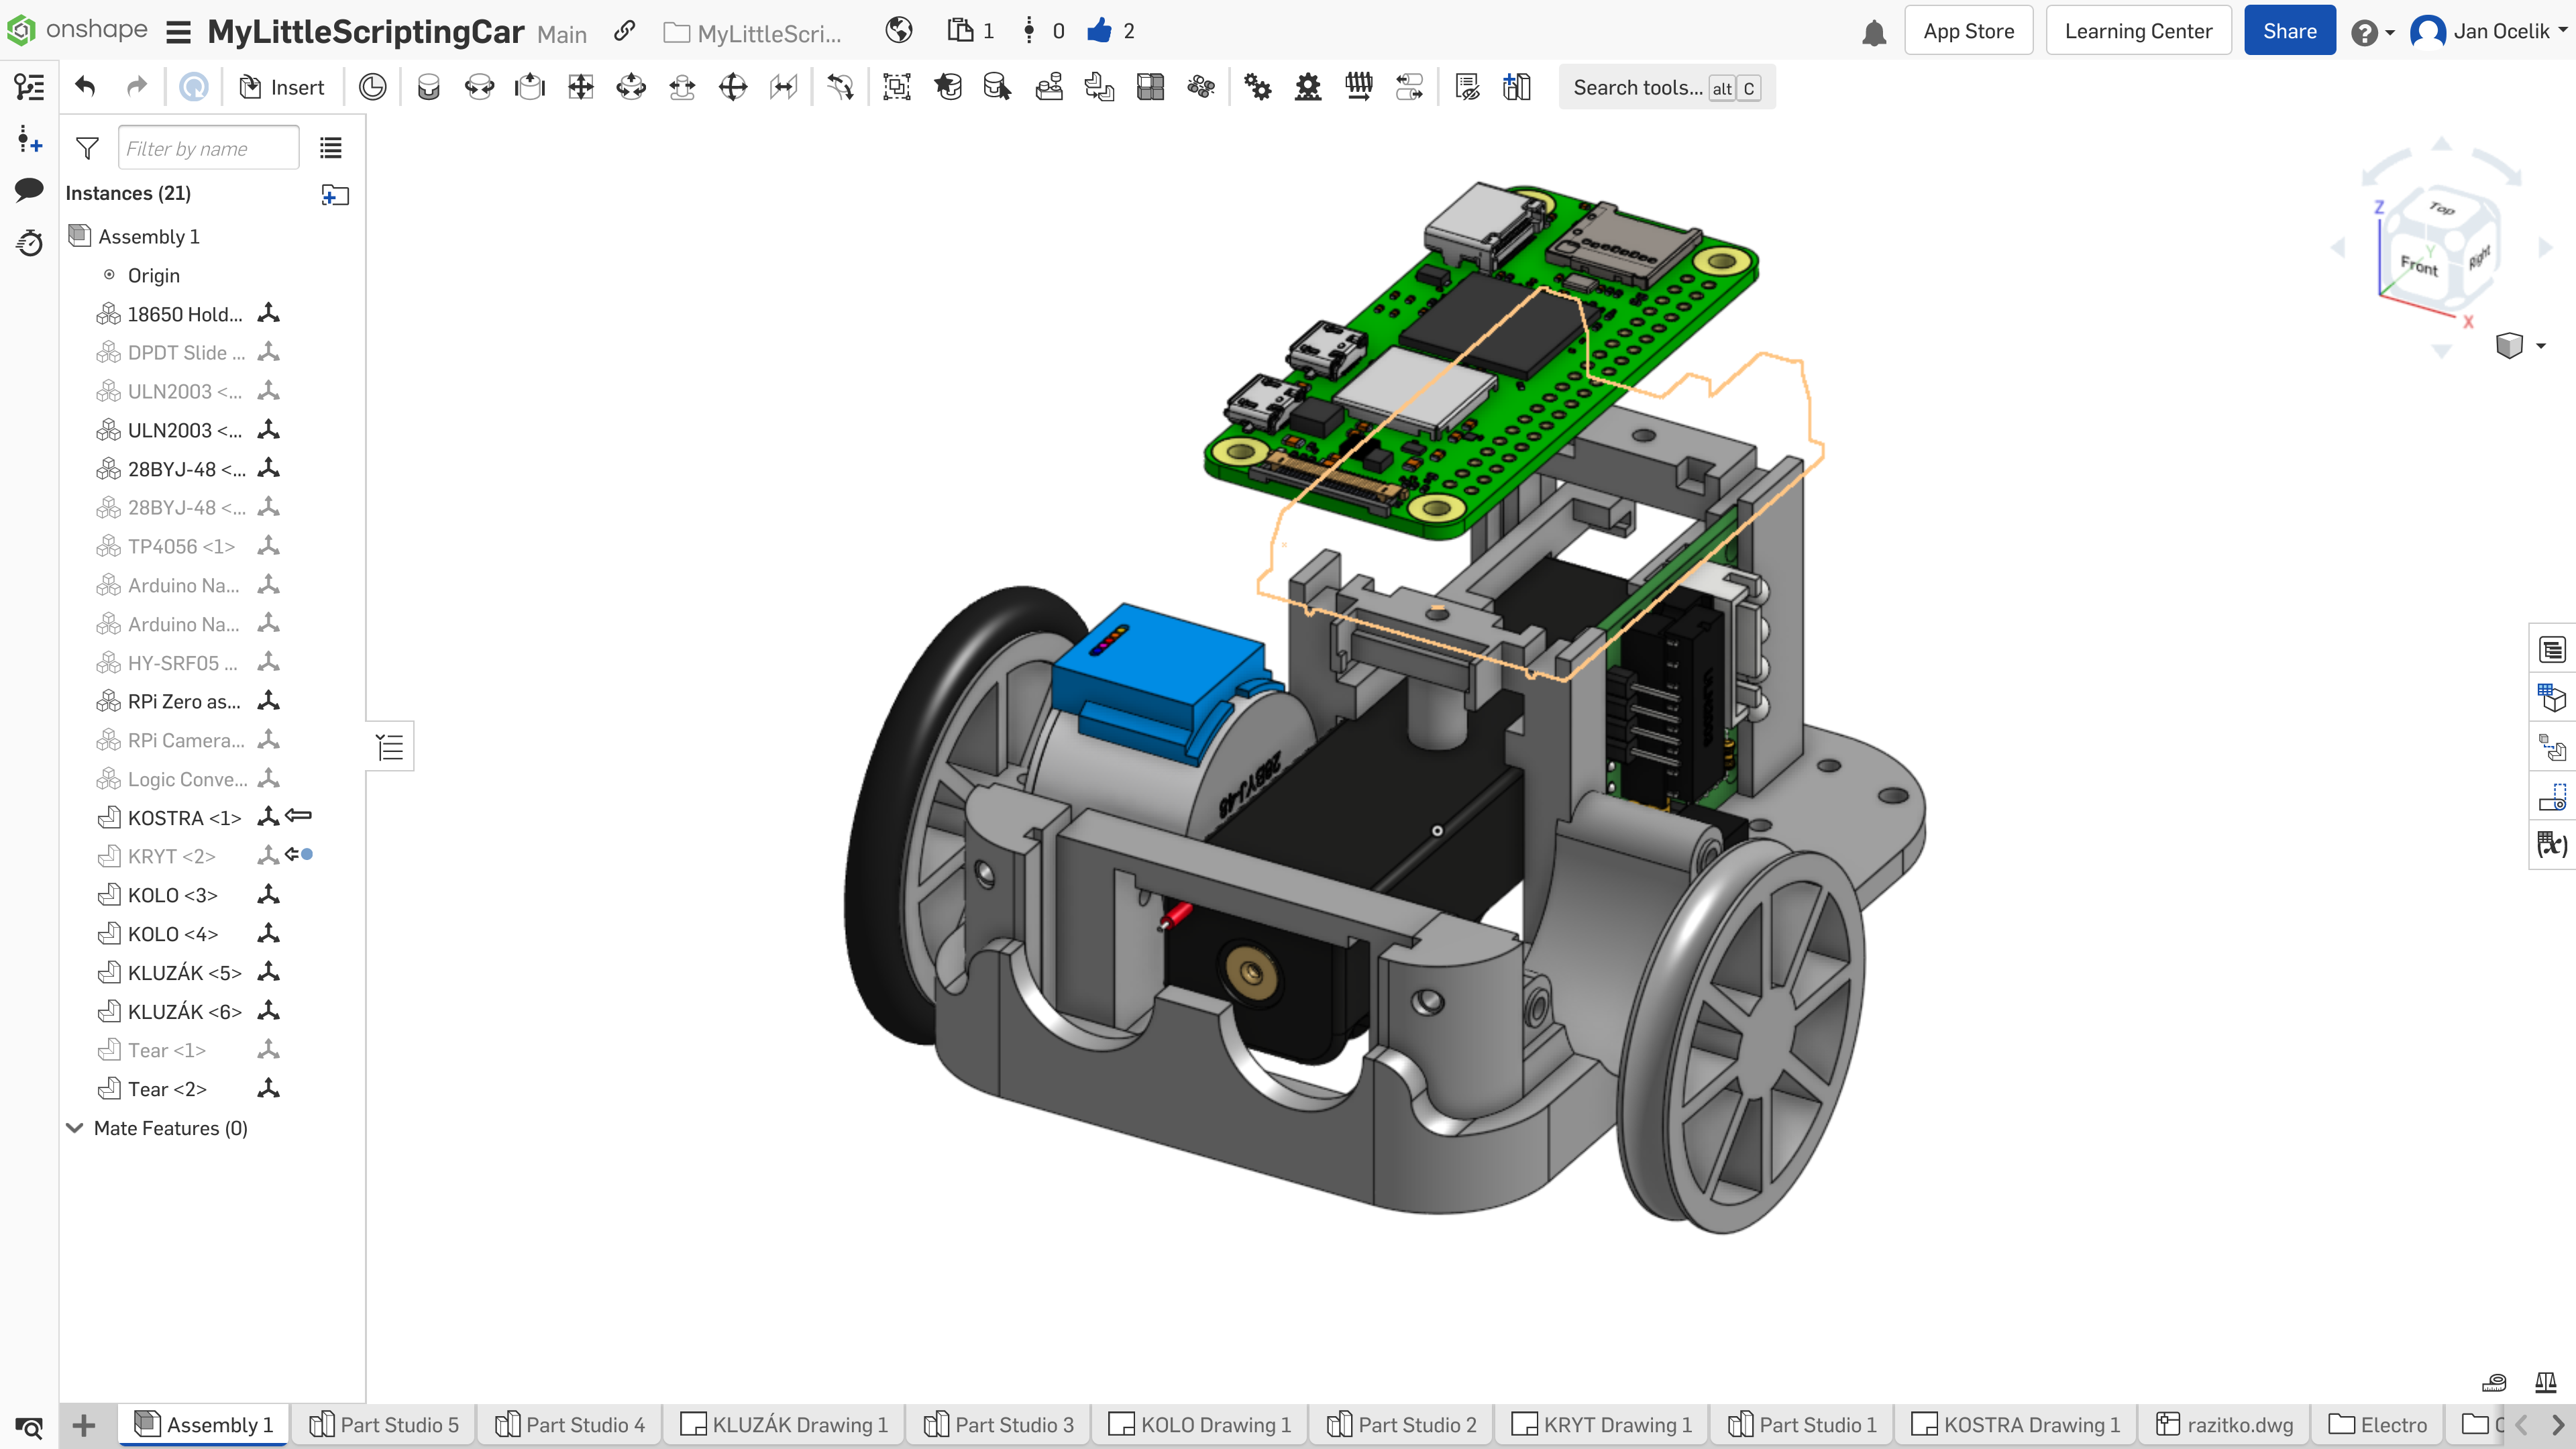
\includegraphics[width=\linewidth]{images/assembly_studio.png}
		\caption{Assembly}
		\label{fig:assembly_studio}
	\end{figure}
	
	\subsubsection*{Drawing}
	\paragraph{} Drawing se dá vyvolat jak samostatně, tak rovnou v kontextu s daným dílem a to jak z Part Stuido, tak z Assembly. Uživateli stačí, kdy v seznamu dílů vybere danou položku a přes kontextové menu vybere možnost \textbf{Create Drawing of...}. Výkres se zde upravuje také pomocí příkazů, stejně jako v předešlých studiích. \textbf{Drawing} studio umožňuje také globální nastavení kót, písma, čar atd.
	
	\begin{figure}[h]
		\centering
		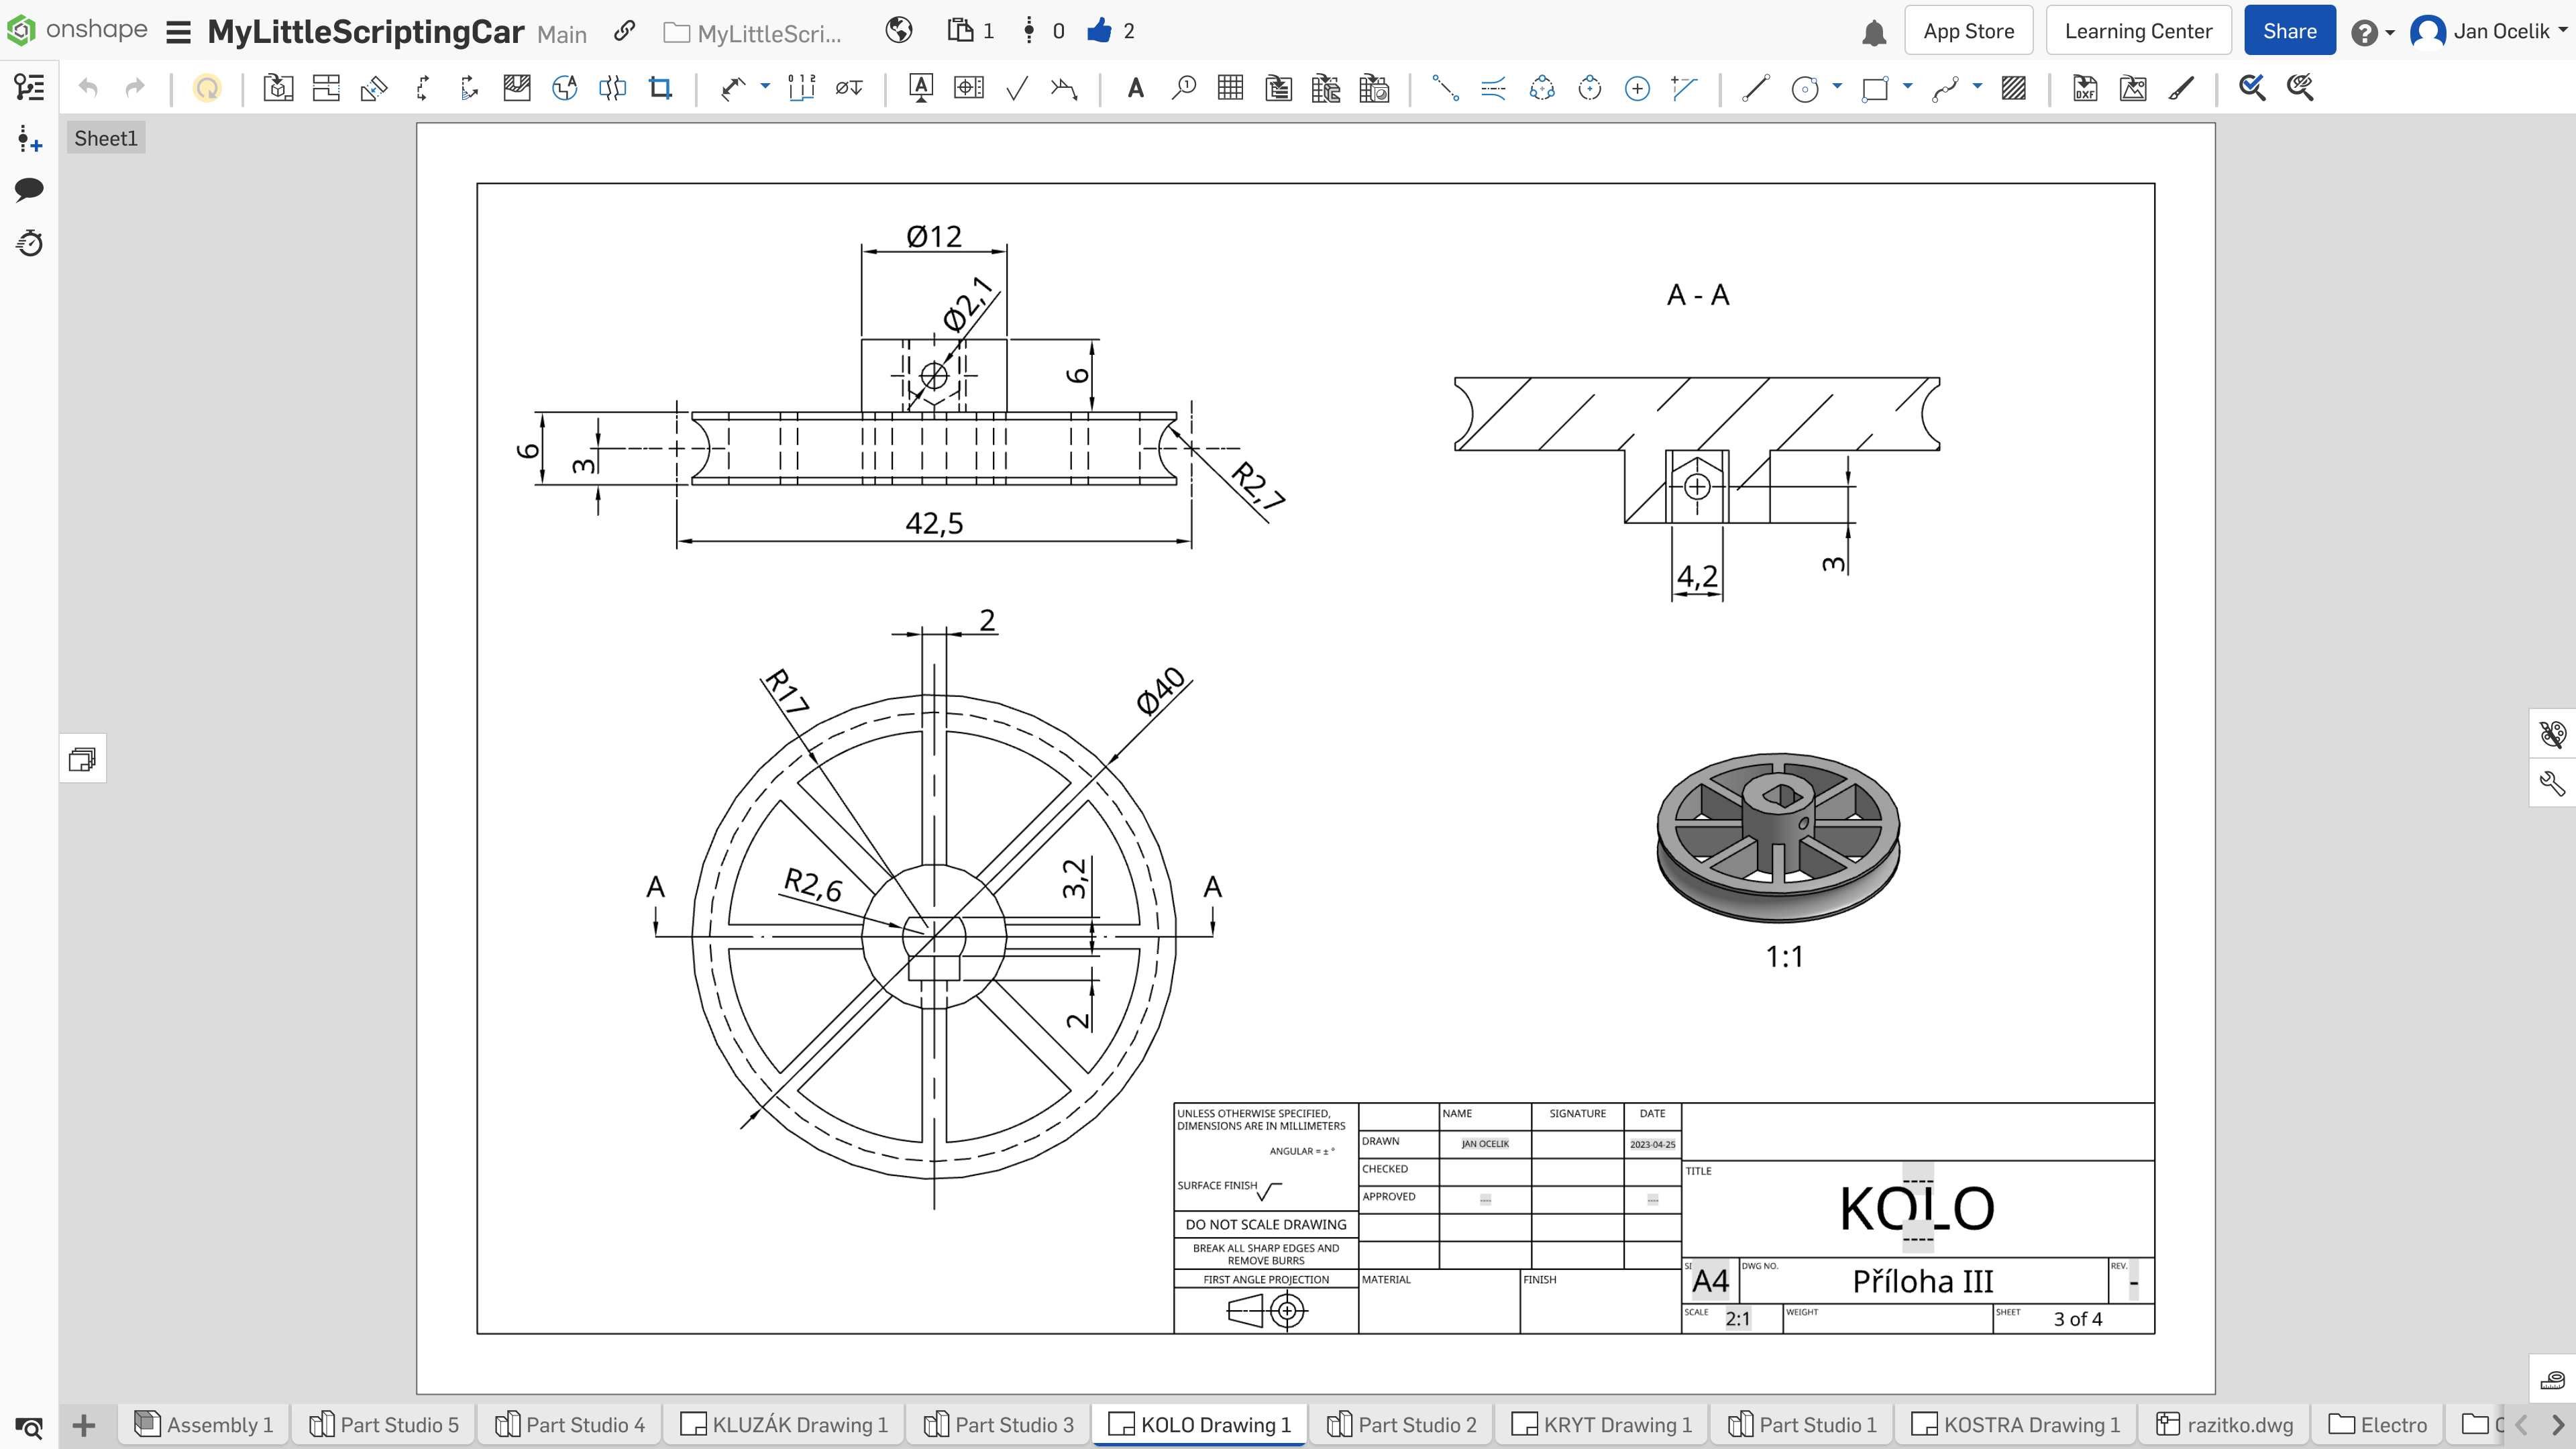
\includegraphics[width=\linewidth]{images/drawing_studio.png}
		\caption{Drawing}
		\label{fig:drawing_studio}
	\end{figure}
	
	\subsection{Code OSS/VS Code}
	\subsubsection{dsadasdas}
	\subsubsection{dasdsadsa}
	\subsubsection{dsadsadsa}
	
\end{spacing}

\end{document}
% Konec dokumentu